\documentclass[a4paper,article,14pt]{extarticle}

\usepackage{spbudiploma}
\usepackage{amsmath}
\usepackage{mathtools}
\usepackage[pdftex]{graphicx}
\graphicspath{{../pictures/}}
\usepackage{listings}
\usepackage{xcolor}

\definecolor{codegreen}{rgb}{0,0.6,0}
\definecolor{codegray}{rgb}{0.5,0.5,0.5}
\definecolor{codepurple}{rgb}{0.58,0,0.82}
\definecolor{backcolour}{rgb}{0.95,0.95,0.92}

\lstdefinestyle{mystyle}{
	backgroundcolor=\color{backcolour},   
	commentstyle=\color{codegreen},
	keywordstyle=\color{codegreen},
	numberstyle=\tiny\color{codegray},
	stringstyle=\color{codepurple},
	basicstyle=\ttfamily\footnotesize,
	breakatwhitespace=false,         
	breaklines=true,                 
	captionpos=b,                    
	keepspaces=false,                 
	numbers=left,                    
	numbersep=5pt,                  
	showspaces=false,                
	showstringspaces=false,
	showtabs=false,                  
	tabsize=2
}

\lstset{style=mystyle}

\begin{document}
	\begin{titlepage}
		\begin{center}
			FEDERAL STATE AUTONOMOUS EDUCATIONAL INSTITUTION
			
			OF HIGHER EDUCATION
			
			ITMO UNIVERSITY
			\vspace{3cm}
			
			\large\textbf{Report}
			
			\large on the practical task No. 1
			
			\large \flqq Experimental time complexity analysis\frqq
			\vspace{5cm}
			

			\begin{flushright}
				{Performed by:} \\
				Putnikov Semyon \\ 
				J4132c \\
			\end{flushright}
			
			
			\begin{flushright}
				{Accepted by:} \\
				Dr Petr Chunaev \\ 
			\end{flushright}
			\vfill
			
			{Санкт-Петербург}
			\par{\number\year}
		\end{center}
	\end{titlepage}

	\newpage
	
	\section{Goal}
	Experimental study of the time complexity of different algorithms.
	
	\section{Formulation of the problem}
	For each n from 1 to 2000, measure the average computer execution time (using timestamps) of programs implementing the algorithms and functions below for five runs. Plot the data obtained showing the average execution time as a function of n. Conduct the theoretical analysis of the time complexity of the algorithms in question and compare the empirical and theoretical time complexities.
	
	\begin{enumerate}
		\item Generate an n-dimensional random vector $\vec{v}$ with non-negative elements. For $\vec{v}$  implement the following calculations and algorithms:
		\begin{enumerate}
			\item \begin{math} f(v) = const \end{math} \textit{(constant function)}
			\item \begin{math} f(v) = \sum_{k=1}^n v_k\end{math} \textit{(the sum of elements)}
			\item \begin{math} f(v) = \prod_{k=1}^n v_k\end{math} \textit{(the product of elements)}
			\item supposing that the elements of $\vec{v}$ are the coefficients of a polynomial \textit{P} of degree n-1, calculate the value \textit{P(1.5)} by a direct calculation of $P(x)=\sum_{k=1}^n v_k x^{k-1}$ (i.e. evaluating each term one by one) and by Horner’s method by representing the polynomial as $P(x)=v_1+x(v_2+x(v_3+...))$;
			\item Bubble Sort of the elements of $\vec{v}$;
			\item Quick Sort of the elements of $\vec{v}$;
			\item Timsort of the elements of $\vec{v}$;
		\end{enumerate}
		\item Generate random matrices \textit{A} and \textit{B} of size $n\times n$ with non-negative elements. Find the usual matrix product for \textit{A} and \textit{B}.
		\item Describe the data structures and design techniques used within the algorithms.
	\end{enumerate}
	
	\section{Brief theoretical part}
	\subsection{Horner's method}
	Horner's method is a method for approximating the roots of polynomials that was described by William George Horner in 1819.
	
	Given the polynomial $p(x)=\sum_{k=1}^n a_i x^i=a_0+a_1 x+a_2 x^2+a_3 x^3+...+a_n x^n$ where $a_0,...a_n$ are constant coefficients, the problem is to evaluate the polynomial at a specific value $x_0$ of $x$.
	
	For this, a new sequence of constants is defined recursively as follows:
	\begin{align}
	b_n &:= a_n \\
	b_{n-1 } &:= a_{n-1}+b_n x_0 \\
	&\vdotswithin{:=} \notag \\
	b_1 &:= a_1+b_2 x_0\\
	b_0 &:= a_0+b_1x_0
	\end{align}
	
	Then $b_0$ is the value of $p(x_0)$. To see why this works, the polynomial can be written in the form 
	\begin{align}
	p(x)=a_0 +x\Bigg(a_1+x\bigg(a_2+x\Big(a_3+...+x\big(a_{n-1} + xa_n\big)...\Big)\bigg)\Bigg)
	\end{align}
	
	\subsection{Bubble sort}
	
	\subsection{Quick sort}
	
	\subsection{Timsort}
	
	\section{Results}
	%Present the results of solving the assigned problems, including graphs and tables, as well as a brief discussion of the results obtained (at most 4 pages)
	\subsection{Constant function (subtask a)}
	\begin{figure}[h]
		\centering
		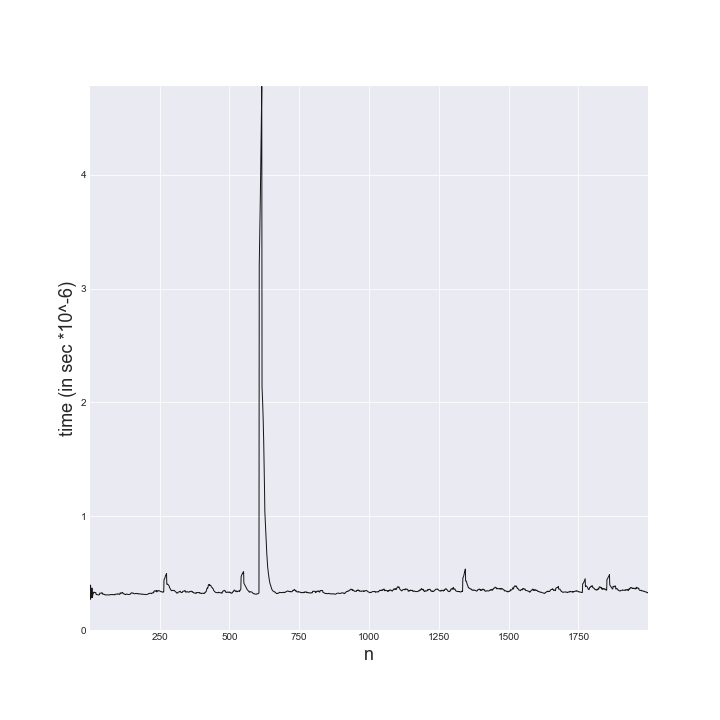
\includegraphics[scale=0.5]{constant.png}
		\caption{Plot of constant function.}
		\label{constant}
	\end{figure} 
	At Figure \ref{constant} we can see execution time of constant function. This plot tends to direct line as expected, but have some outliers. It is a result of cpu overheating which affects execution process.
	
	Nevertheless, the graph proofs that the execution time of constant function does not depend on the number of variables.
	

	\subsection{The sum of elements (subtask b)}
	\ref{sum}
	\begin{figure}[h]
		\centering
		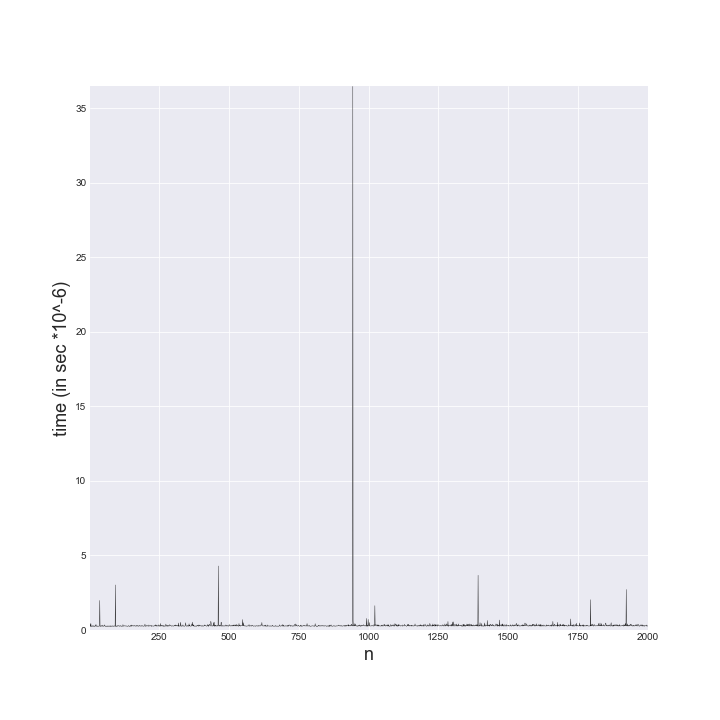
\includegraphics[scale=0.5]{sumOfVector.png}
		\caption{Plot for sum of elements.}
		\label{sum}
	\end{figure} 

	\subsection{The product of elements (subtask c)}
	\ref{product}
	\begin{figure}[h]
		\centering
		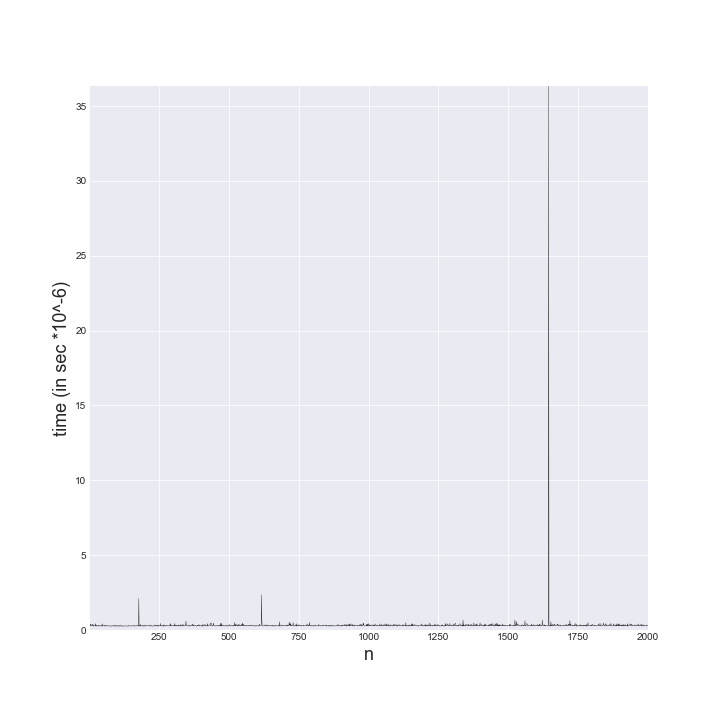
\includegraphics[scale=0.5]{productOfVector.png}
		\caption{Plot for product of elements.}
		\label{product}
	\end{figure} 
	
	\subsection{Polynom calculation (subtask d)}
	\ref{direct}
	\ref{horners}
	\begin{figure}[h]
		\centering
		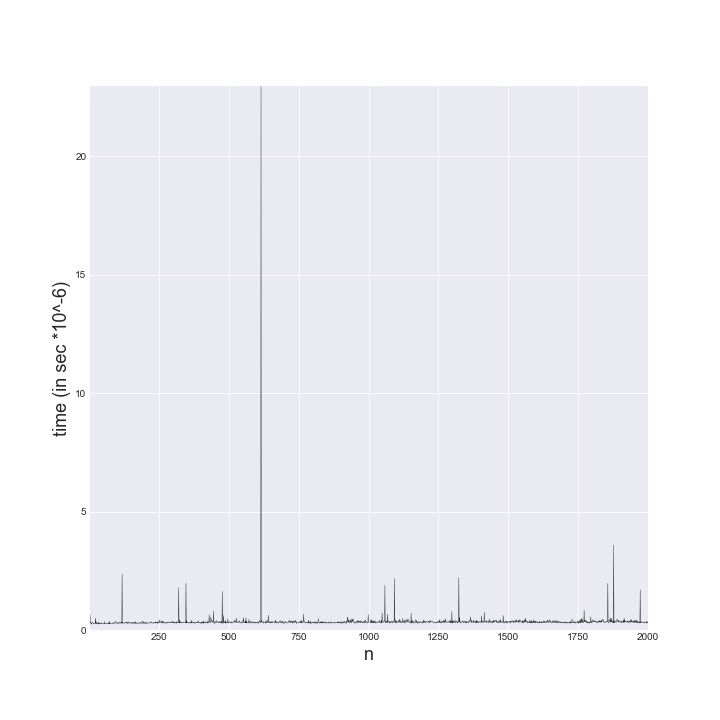
\includegraphics[scale=0.5]{calculatePolinom.png}
		\caption{Plot for direct polinom calculation.}
		\label{direct}
	\end{figure} 

	\begin{figure}
		\centering
		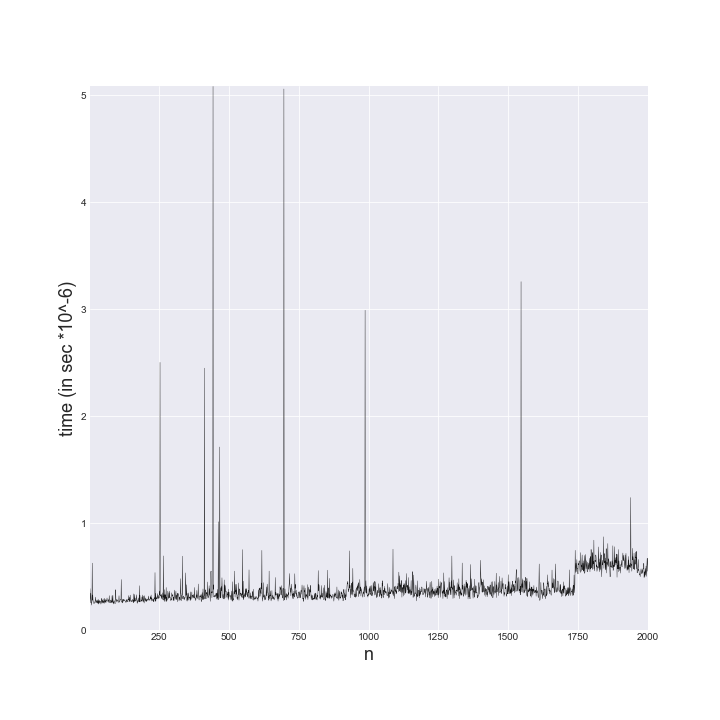
\includegraphics[scale=0.5]{horners.png}
		\caption{Plot for polinom calculation by Horner's method.}
		\label{horners}
	\end{figure} 
	
	
	\section{Conclusions}
	%Make conclusions on the results obtained and on the achievement of the goal of your work
	
	\section{Appendix}
	%Present the listings of programs written for performing the task, with comments
	\begin{lstlisting}[language=Python, caption=Constant function]
	def constant(vector,value): 
		return 0
	\end{lstlisting}
	
	\begin{lstlisting}[language=Python, caption=Sum of elements]
	def sumOfVector(vector, value):
		return sum(vector)
	\end{lstlisting}
	
	\begin{lstlisting}[language=Python, caption=Product of elements]
	def productOfVector(vector, value):
		return numpy.prod(vector)
	\end{lstlisting}
	
	\begin{lstlisting}[language=Python, caption=Direct polinom calculation]
	def calculatePolinom(vector, value):
		result = 0
		power = 0
		for item in vector:
			result += item*(value**power)
			power += 1
		return result
	\end{lstlisting}
	
	\begin{lstlisting}[language=Python, caption=Polinom calculation by Horner's method]
	def horners(vector,value):
		v = list(vector)
		v.reverse()
		def hRec(v, value):
			if (len(v)==1):
				return v.pop()
			else:
				return v.pop() + value*hRec(v,value)
		return hRec(v,value)
	\end{lstlisting}
	
	\begin{lstlisting}[language=Python, caption=Bubble sort]
	def bubbleSort(vector,value):
		array = list(vector)
		size = len(array)
		for i in range(size-1):
			for j in range(size-i-1):
				if array[j] > array[j+1]:
					array[j], array[j+1] = array[j+1], array[j]
		return array
	\end{lstlisting}
	
	\begin{lstlisting}[language=Python, caption=Bubble sort]
	def quickSort(vector, value):
		array = list(vector)
		if len(array) <= 1:
			return array
		else:
			q = random.choice(array)
			s_nums = []
			m_nums = []
			e_nums = []
			for n in array:
				if n < q:
					s_nums.append(n)
				elif n > q:
					m_nums.append(n)
				else:
					e_nums.append(n)
			return quickSort(s_nums, value) + e_nums + quickSort(m_nums, value)
	\end{lstlisting}
	
	
	
\end{document}